\input{header.tex}

\subject{V201}
\title{Das Dulong-Petitsche Gesetz}
\date{
  Durchführung: 18.01.2019
  \hspace{3em}
  Abgabe: 25.01.2019
}

\begin{document}

\maketitle
\thispagestyle{empty}
\tableofcontents
\newpage

\input{Theorie/theorie.tex}
%\newpage
\section{Aufbau und Durchführung}
Das Viskosimeter nach Höppler besteht hauptsächlich aus zwei Bestandteilen und ist in Abbildung \ref{fig:a} dargestellt.
Das wichtigste Element ist das Fallrohr, in dem sich die zu untersuchende Flüssigkeit und die Kugel befinden.
An beiden Enden des Fallrohrs ist eine Öffnung, die durch Stopfen und Schrauben luftdicht verschlossen werden, nachdem die oben genannten Materialien in das Fallrohr gegeben werden.
Dabei sollte darauf geachtet werden, dass in der Flüssigkeit keine Luftbläschen vorhanden sind um das Messergebnis nicht zu verfälschen.
Der zweite Bestandteil ist das um das Fallrohr befindliche, aber räumlich getrennte, Wasserbad, welches erwärmt bzw. abgekühlt wird und dessen Temperatur durch das Thermostat eingestellt werden kann.
Ein angebrachtes Thermometer zeigt die Temperatur der Flüssigkeit im Fallrohr.
Während des Versuchs wird die Einrichtung minimal gekippt, damit die Kugel keine turbulenten Ströme auslöst und das Messergebnis ungenauer wird.
An dem Fallzylinder sind Messmarken angebracht um die zurückgelegte Strecke zu überprüfen.
Dabei sollte darauf geachtet werden, die Kugel erst eine annähernd konstante Geschwindigkeit erreichen zu lassen.
Nach einer Messung kann das Viskosimeter durch eine Drehapparatur, die Libelle, um $180°$ gedreht werden und eine weitere Messung durchgeführt werden.
Es werden die Zeiten gemessen, die die Kugel für eine gleichbleibenden Strecke benötigt, und ausgewertet.
Während des Versuchs werden für zwei unterschiedlich schwere Kugeln gleichen Materials die Fallzeiten für die gleichen Zeiten gemessen.
Außerdem wird die Fallzeit für die Größere der beiden Kugeln gemessen, wobei die Temperatur nach zwei Messungen verändert wird.
Dabei wird die Temperatur der äußeren Flüssigkeit aufgeheizt, wodurch auch das destillierte Wasser im Fallrohr erwärmt wird.
Es werden jeweils zwei Zeiten für zehn verschiedene Temperaturen gemessen.
\begin{figure}[H]
    \centering
    \caption{Das Fallviskosimeter nach Höppler}
    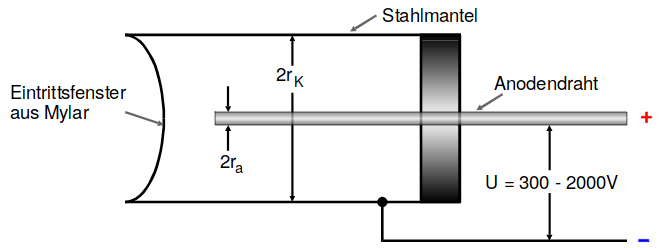
\includegraphics[height=8cm]{Aufbau.png}
    \label{fig:a}
\end{figure}

\section{Durchführung}

\subsection{Der A-Scan}
Zunächst sollen mit Hilfe des A-Scans die Störstellen des Acrylblocks, der in Abbildung \ref{fig:acryl} dargestellt ist, identifiziert werden.
Dazu wird mit einer $\SI{1}{MHz}$-Sonde die Lage der Bohrungen untersucht.
Dabei und bei den folgenden Messungen sollte Wasser als Kontaktmittel verwendet werden, da Luft einen sehr hohen Absorptionskoeffizienten hat.
Die Sonde wird über die Störstellen gesetzt und die Laufzeit gemessen.
Danach wird die Messung von der anderen Seite wiederholt um die Dicke der Störstellen zu bestimmen.
Es muss die Laufzeitkorrektur aufgrund des Kontaktmittels berücksichtig werden.

\subsection{Das Auflösungsvermögen}
In der nächsten Messung werden Sonden von $\SI{1}{MHz}$, $\SI{2}{MHz}$ und $\SI{4}{MHz}$ verwendet.
Dann werden die Störstellen 1 und 2 jeweils untersucht und Messungen mit dem A-Scan aufgenommen.

\subsection{Der B-Scan}
Bei dieser Messung wird mit einer $\SI{2}{MHz}$-Sonde der B-Scan durchgeführt.
Dabei wird die Sonde langsam und konstant über den Acrylblock bewegt um ein gleichmä\ss{}iges Bild zu erhalten.
Dann werden jeweils die Messzeitdifferenzen der Störstellen notiert.
Daraufhin wird der Acrylblock umgedreht und die Messung wiederholt.

\subsection{Der TM-Scan}
Es wird ein einfaches Herzmodell untersucht, das aus einem Doppelgefä\ss{} und einer beweglichen Membran besteht.
Dabei kann die Membran eigenständig durch einen Gummiball bewegt werden.
Aus der Messung werden dann aus dem enddiastolischen und das endsystolischen Volumen das Herzvolumen bestimmt.
Dazu wird der obere Behälter zur Hälfte mit Wasser gefüllt.
Mit einer $\SI{2}{MHz}$-Sonde wird dann bei regelmä\ss{}igem Aufpumpen der Membran ein TM-Scan des Herzens gemacht.
Dabei sollte die Sonde auf der Wasseroberfläche angebracht sein.

\begin{figure}[h]
    \centering
    \includegraphics[height=5cm]{Durchführung/Objekt.pdf}
    \caption{Der Acrylblock. \cite{US2}}
    \label{fig:acryl}
\end{figure}
\section{Auswertung}
\label{Auswertung}
\subsection{Charakteristik}
Die bei der Messung aufgenommenen Zählraten $N$ sind in Tabelle \ref{tab:Messung1} aufgetragen. Diese werden in Abhängigkeit von der Spannung $U$ bei einer jeweiligen Messzeit von 60 s aufgenommen und auf 1 s umgerechnet. \*
Der Fehler von $N$ ergibt sich dabei durch
\begin{equation*}
	\increment N = \sqrt{N}.
\end{equation*}

\begin{table} [H]
	\centering
	\caption{Messdaten der Charakteristik des Zählrohres.}
	\label{tab:Messung1}
	\sisetup{table-format=4.2}
	\begin{tabular}{S[table-format=4.2]ccc}
		\toprule
		{$U / V$}&{$N / s$}&{$I / \mu A$} \\
		\midrule
		300& 0& 0\\
		310 &190.17$\pm$13.79& 0.1\\
		320 &196.10$\pm$14.00& 0.1\\
		330 &199.20$\pm$14.11& 0.1\\
		340 &196.02$\pm$14.00& 0.1\\
		350 &199.15$\pm$14.11& 0.2\\
		360 &199.70$\pm$14.13& 0.2\\
		370 &202.40$\pm$14.23& 0.2\\
		380 &200.50$\pm$14.16& 0.3\\
		390 &202.08$\pm$14.22& 0.3\\
		400 &202.62$\pm$14.23& 0.3\\
		410 &204.47$\pm$14.30& 0.3\\
		420 &204.22$\pm$14.29& 0.4\\
		430 &205.55$\pm$14.34& 0.4\\
		440 &203.50$\pm$14.27& 0.4\\
		450 &203.60$\pm$14.27& 0.4\\
		460 &206.78$\pm$14.38& 0.5\\
		470 &207.67$\pm$14.41& 0.5\\
		480 &203.88$\pm$14.28& 0.5\\
		490 &205.08$\pm$14.32& 0.6\\
		500 &205.62$\pm$14.34& 0.6\\
		510 &205.67$\pm$14.34& 0.6\\
		520 &207.02$\pm$14.39& 0.6\\
		530 &208.18$\pm$14.43& 0.7\\
		540 &206.93$\pm$14.39& 0.7\\
		550 &206.95$\pm$14.39& 0.7\\
		560 &204.08$\pm$14.29& 0.7\\
		570 &208.63$\pm$14.44& 0.8\\
		580 &207.05$\pm$14.39& 0.8\\
		590 &205.38$\pm$14.33& 0.8\\
		600 &210.23$\pm$14.50& 0.8\\
		610 &204.50$\pm$14.30& 0.9\\
		620 &208.87$\pm$14.45& 1.0\\
		630 &210.90$\pm$14.52& 1.0\\
		640 &206.82$\pm$14.38& 1.0\\
		650 &211.22$\pm$14.53& 1.0\\
		660 &212.85$\pm$14.59& 1.0\\
		670 &213.13$\pm$14.60& 1.0\\
		680 &217.32$\pm$14.74& 1.1\\
		690 &214.05$\pm$14.63& 1.1\\
		700 &220.70$\pm$14.86& 1.2\\
		\bottomrule 
	\end{tabular}
\end{table} 

In Abbildung \ref{fig:Charakteristik} ist die Charakteristik des Zählrohres abgebildet. Hierzu wurde Zählrate pro Sekunde verwendet ($N \cdot \frac{1}{\text{s}}$). Die Fehler ergeben sich durch
\begin{equation*}
	\increment n = \frac{\sqrt{N}}{\increment t}
\end{equation*}

\begin{figure}[H]
    \centering
    \includegraphics[scale=0.7]{Auswertung/Charakteristik.pdf}
    \caption{Charakteristik des Zählrohres.}
    \label{fig:Charakteristik}
\end{figure}

Es ist zu erkennen, dass das Plateau erst bei einer Spannung von 310 V besteht. Um dieses Plateau nun genauer zu untersuchen, wird eine lineare Regression ab einer Spannung von 310 V durchgeführt. Diese ist in Abbildung \ref{fig:Regression} abgebildet. 

\begin{figure}[H]
    \centering
    \includegraphics[scale=0.7]{Auswertung/Charakteristik_Regression.pdf}
    \caption{Regression des Charakteristik-Plateaus.}
    \label{fig:Regression}
\end{figure}

Als Regressionsfunktion wurde 
\begin{equation*}
	I(U) = m \cdot U + b
\end{equation*}
verwendet.
Es ergeben sich folgende Werte:
\begin{gather*}
	m = 0.02051 \pm 0.00003 \frac{1}{\text{Vs}} \\
	b = 196 \pm 7 \frac{1}{\text{s}}\\
\end{gather*}
Somit ergibt sich eine Plateausteigung von
\begin{equation*}
	m_\text{Pl} = (1 \pm 0.00005)\%  \text{pro}  100V .
\end{equation*}

\subsection{Totzeit}
\subsubsection{Ablesen des Oszilloskops}
Am Oszilloskop lassen sich folgende Totzeiten $T_\text{t}$ und Erholungszeiten $T_\text{E}$ ablesen:
  
\begin{table} [H]
	\centering
	\caption{Totzeiten $T_\text{t}$ und Erholungszeiten $T_\text{E}$ des Zählrohres.}
	\label{tab:Zeiten}
	\sisetup{table-format=4.2}
	\begin{tabular}{S[table-format=4.2]|cc}
		\toprule
		{$U / V$}&{$T_\text{t} / \mu s$}&{$T_\text{E} / \mu s$} \\
		\midrule
		550&60$\pm$1&140$\pm$1\\
		500&58$\pm$1&120$\pm$1\\
		450&56$\pm$1&100$\pm$1\\
		\bottomrule 
	\end{tabular}
\end{table} 
	
Die Fehler ergeben sich, da ein genaues Ablesen nicht möglich ist.
Aus den berechneten Werten wird dann der Mittelwert mit folgender Formel gebildet.
\begin{equation*}
    \overline{x} = \frac{1}{N} \sum_{i=1}^N x_i
\end{equation*}

Somit ergibt sich nach dieser Messung eine Totzeit und eine Erholungszeit von:
\begin{gather*}
	 T_\text{t} =  58\pm1 \\
	T_\text{E} = 120\pm1
\end{gather*}

\subsubsection{Zwei-Quellen-Methode}
Bei der Zwei-Quellen-Methode werden folgende Zählraten innerhalb von 60 Sekunden, bei einer Spannung $U$ von 450V, gemessen:

\begin{table} [H]
	\centering
	\caption{Totzeiten $T_\text{t}$ und Erholungszeiten $T_\text{E}$ des Zählrohres.}
	\label{tab:Zeiten}
	\sisetup{table-format=10}
	\begin{tabular}{|ccc|}
		\toprule
		{$\frac{N_1}{60\text{s}}$}&{$\frac{N_2}{60\text{s}}$}&{$\frac{N_{1+2}}{60\text{s}}$} \\
		\midrule
		14034$\pm$118&13155$\pm$115&26491$\pm$163\\
		\bottomrule 
	\end{tabular}
\end{table} 

Durch Gleichung 
\begin{equation*}
	T = \frac{N_1 + N_2 - N_{1+2}}{2N_1N_2}
\end{equation*}
ergibt sich somit für die Totzeit der Wert:
\begin{equation*}
	T_\text{t} = \SI{19\pm6}{\second}
\end{equation*}

Der Fehler lässt sich nach der Gaußschen Fehlerfortpflanzung bestimmen:
\begin{equation*}
  \begin{split}
  \increment T = & \biggl(\left(\frac{2n_1n_2 - (n_1+n_2-n_{1+2})2n_2}{(2n_1n_2)^2}\cdot \increment n_1 \right)^2 \\
  + & \left(\frac{2n_1n_2 - (n_1+n_2-n_{1+2})2n_1}{(2n_1n_2)^2} \cdot \increment n_2\right)^2  +  \left(-\frac{2n_1n_2}{(2n_1n_2)^2} \cdot \increment n_{1+2}\right)^2\biggr)^{\frac{1}{2}}.
  \end{split}
\end{equation*}

\subsection{Freigesetzte Ladung}
Die zur Bestimmung der Ladung benötigten Messwerte sind in Tabelle \ref{tab:Messung2} aufgetragen. 

\begin{table} [h]
	\centering
	\caption{Messdaten der Charakteristik des Zählrohres.}
	\label{tab:Messung2}
	\sisetup{table-format=4.2}
	\begin{tabular}{S[table-format=4.2]ccc}
		\toprule
		{$U / V$}&{$N / s$}&{$I / \mu A$}&{$Q \cdot 10^{10} / e_0$} \\
		\midrule
		300& 0& 0 &0\\
		310 &190.17$\pm$13.79& 0.1&3.28$\pm$0.030 \\
		320 &196.10$\pm$14.00& 0.1&3.18$\pm$0.029\\
		330 &199.20$\pm$14.11& 0.1&3.13$\pm$0.028\\
		340 &196.02$\pm$14.00& 0.1&3.18$\pm$0.029\\
		350 &199.15$\pm$14.11& 0.2&6.27$\pm$0.061\\
		360 &199.70$\pm$14.13& 0.2&6.25$\pm$0.061\\
		370 &202.40$\pm$14.23& 0.2&6.17$\pm$0.060\\
		380 &200.50$\pm$14.16& 0.3&9.34$\pm$0.082\\
		390 &202.08$\pm$14.22& 0.3&9.27$\pm$0.081\\
		400 &202.62$\pm$14.23& 0.3&9.24$\pm$0.081\\
		410 &204.47$\pm$14.30& 0.3&9.16$\pm$0.081\\
		420 &204.22$\pm$14.29& 0.4&12.2$\pm$0.111\\
		430 &205.55$\pm$14.34& 0.4&12.1$\pm$0.112\\
		440 &203.50$\pm$14.27& 0.4&12.3$\pm$0.112\\
		450 &203.60$\pm$14.27& 0.4&12.3$\pm$0.112\\
		460 &206.78$\pm$14.38& 0.5&15.1$\pm$0.124\\
		470 &207.67$\pm$14.41& 0.5&15.0$\pm$0.124\\
		480 &203.88$\pm$14.28& 0.5&15.3$\pm$0.126\\
		490 &205.08$\pm$14.32& 0.6&18.3$\pm$0.132\\
		500 &205.62$\pm$14.34& 0.6&18.2$\pm$0.132\\
		510 &205.67$\pm$14.34& 0.6&18.2$\pm$0.132\\
		520 &207.02$\pm$14.39& 0.6&18.1$\pm$0.132\\
		530 &208.18$\pm$14.43& 0.7&21.0$\pm$0.252\\
		540 &206.93$\pm$14.39& 0.7&21.1$\pm$0.252\\
		550 &206.95$\pm$14.39& 0.7&21.1$\pm$0.252\\
		560 &204.08$\pm$14.29& 0.7&21.4$\pm$0.255\\
		570 &208.63$\pm$14.44& 0.8&23.9$\pm$0.289\\
		580 &207.05$\pm$14.39& 0.8&24.1$\pm$0.290\\
		590 &205.38$\pm$14.33& 0.8&24.3$\pm$0.292\\
		600 &210.23$\pm$14.50& 0.8&23.8$\pm$0.289\\
		610 &204.50$\pm$14.30& 0.9&27.5$\pm$0.301\\
		620 &208.87$\pm$14.45& 1.0&29.9$\pm$0.333\\
		630 &210.90$\pm$14.52& 1.0&29.6$\pm$0.331\\
		640 &206.82$\pm$14.38& 1.0&30.2$\pm$0.334\\
		650 &211.22$\pm$14.53& 1.0&29.6$\pm$0.331\\
		660 &212.85$\pm$14.59& 1.0&29.3$\pm$0.329\\
		670 &213.13$\pm$14.60& 1.0&29.3$\pm$0.329\\
		680 &217.32$\pm$14.74& 1.1&31.6$\pm$0.360\\
		690 &214.05$\pm$14.63& 1.1&32.1$\pm$0.382\\
		700 &220.70$\pm$14.86& 1.2&33.9$\pm$0.398\\
		\bottomrule 
	\end{tabular}
\end{table} 

Der Fehler ergibt sich dabei durch 
\begin{equation*}
	\increment Q = \frac{I}{e_0 N^2}
\end{equation*} 
\section{Diskussion}
Zunächst lässt sich sagen, dass die Bragg-Bedingung aufgrund der geringen Abweichung als erfüllt angesehen werden kann.
Es wurde anstatt eines Maximums bei einem Winkel von $\theta_\text{theo} = \SI{14}{°}$ ein Winkel von $\theta_\text{exp} = \SI{14.35}{°}$ gemessen.
Das ergibt eine Abweichung von $2,5 \%$.

Für die drei Abschirmkonstanten ergeben sich
\begin{equation}
    \sigma_1 = 3,375  \qquad \text{,} \qquad \sigma_2 = 12,727 \qquad \text{und} \qquad \sigma_3 = 28,545. \notag
\end{equation}

Des Weiteren wurden die Abschirmkonstanten der K-Linien von Gallium, Zink, Zirkonium und Brom bestimmt.
Die dazu notwendigen Energien sind in Tabelle \ref{tab:ene} aufgelistet.

\begin{table}[H]
    \begin{center}
      \caption{Messergebnisse der Energien der K-Kante.}
      \label{tab:ene}
      \begin{tabular}{c|c|c|c} 
        \textbf{Material} & \textbf{$E_\text{K,exp}$} & \textbf{$E_\text{K,theo}$} & \textbf{relative Abweichung [$\%$]}\\
        \hline
          \text{Gallium}    & 10,372 & 10,377 & 0,1\\
          \text{Zink}       & 9,670 & 9,668 & 0,2 \\
          \text{Zirkonium}  & 17,939 & 18,008 & 0,4\\
          \text{Brom}       & 13,507 & 13,483 & 0,2 \\
      \end{tabular}
    \end{center}
\end{table}

Für alle experimentell bestimmten Energien der K-Kanten lässt sich sagen, dass die Abweichungen sehr gering sind und die Messung somit aussagekräftig ist.
Für die resultierenden Abschirmkonstanten, die in Tabelle \ref{tab:werte} dargestellt sind, ergaben sich aber durch Näherungen bei der Rechnung größere Fehler.
Dies ist auf Ablesefehler und auf die jeweiligen Absorber zurückzuführen.
\begin{table}[H]
    \begin{center}
      \caption{Messergebnisse der Abschirmkonstanten.}
      \label{tab:werte}
      \begin{tabular}{c|c|c|c} 
        \textbf{Material} & \textbf{$\sigma_\text{1,exp}$} & \textbf{$\sigma_\text{1,theo}$} & \textbf{relative Abweichung [$\%$]}\\
        \hline
          \text{Gallium}    & 3,162 & 3,151 & 0,35 \\
          \text{Zink}       & 3,134 & 3,560 & 11,9 \\
          \text{Zirkonium}  & 3,251 & 4,080 & 21,2 \\
          \text{Brom}       & 3,170 & 3,830 & 17,2 \\
      \end{tabular}
    \end{center}
\end{table}

\subsection{Der schwere Absorber}
Für den schweren Absorber, in diesem Fall Wismut mit einer Kernladungszahl von $z = 83$ wurden die L-Kanten untersucht.
In dem vorliegenden Messbereich wurden die $L_\text{II}$ und die $L_\text{III}$-Kanten untersucht.
Dabei wurden die Werte
\begin{equation}
    E_\text{LII} = \SI{15,470}{keV} \qquad \text{und} \qquad E_\text{LIII} = \SI{13,212}{keV}
\end{equation}
gemessen und mit den Literaturwerten
\begin{equation}
    E_\text{LII,Lit} = \SI{15,711}{keV} \qquad \text{und} \qquad E_\text{LIII,Lit} = \SI{13,419}{keV}
\end{equation}
verglichen.
Dabei ergaben sich Abweichungen von jeweils $1,6 \%$.
Diese Abweichung lassen sich auf Fehler statistischen Ursprungs, des Ablesens und den Absorber zurückführen.
Trotzdem haben die beiden gemessenen Werte eine hohe Aussagekraft.

\subsection{Das Moseleysche Gesetz}
Bei der Untersuchung des Moseleyschen Gesetzes wurde die Rydbergenergie auf
\begin{equation}
    R_\infty = \SI{12,769}{eV}  \notag
\end{equation}
bestimmt.
Zu dem Literaturwert von $R_\text{$\infty$,Lit} = \SI{13,6}{eV}$ hat der ermittelte Wert eine Abweichung von $6,2 \%$.
Es lässt sich sagen, dass die lineare Regression sehr genau war, da der Fehler 5 Größenordnungen unter dem eigentlichen Wert lag.
Außerdem lässt sich sagen, dass der Fehler der Rydbergenergie einerseits auf die geringe Anzahl der Messwerte zurückzuführen ist.
Andererseits natürlich auch auf die Tatsache, dass das eigentliche Ergebnis der Steigung aus der linearen Regression noch quadriert werden musste, wodurch sich auch die Abweichung quadratisch vergrö\ss{}ert.
 
\section{Literatur}

[1] TU Dortmund. Versuchsanleitung zum Experiment V504 - Thermische Elektronenemission. 2019.

[2] https://de.wikipedia.org/wiki/Austrittsarbeit. 19.04.2019

\printbibliography{}

\end{document}